\section{Umsetzung des realen Clusters}
\label{sec:realCluster}

Da mithilfe der Plattform Hadoop"=Benchmark ein komplettes Hadoop"=Cluster auf einem PC ausgeführt werden kann und dieses speziell für die Forschung entwickelt wurde, wurde die Plattform für diese Fallstudie als Basis genutzt
Da Docker und Hadoop vor allem für den Einsatz in einer Linux"=Umgebung entwickelt wurden, werden für die Fallstudie zwei physische Hosts genutzt, auf denen das Cluster wahlweise auf einem oder auf beiden Hosts ausgeführt werden kann.
Zudem wird auf einem Host eine VM mit Windows 10 ausgeführt, das zum Ausführen des .NET"=Frameworks bzw. \ac{ss} benötigt wird.
Beide zum Einsatz kommenden Hosts sind jeweils mit einem Intel Core i5"=4570 @ 3,2 GHz x 4, 16 GB Arbeitsspeicher sowie einer SSD ausgestattet, auf der Ubuntu 16.04 LTS installiert ist.
Die Verbindung von Windows zu Linux auf beiden Hosts wird mithilfe von SSH"=Verbindungen umgesetzt.
Um den Ressourcenbedarf durch die von docker"=machine erzeugten VMs zu reduzieren, werden die Docker"=Container direkt auf den physischen Hosts ausgeführt:

\begin{figure}[h]
    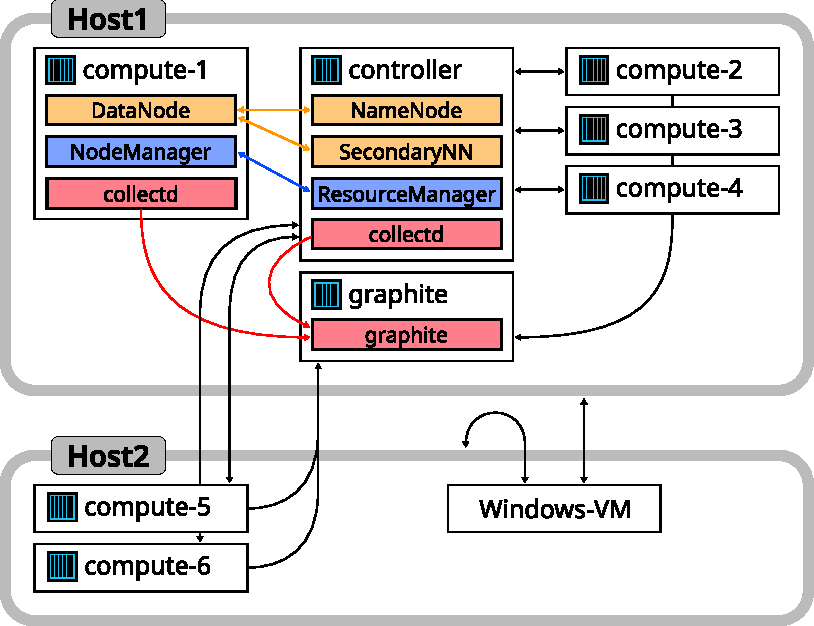
\includegraphics{./resources/caseStudyHadoopSetup.pdf}
    \caption[In der Fallstudie verwendetes Cluster"=Setup]
    {In der Fallstudie verwendetes Cluster"=Setup.
        Grün: \ac{HDFS}, Blau: YARN, Rot: Graphite.}
    \label{fig:caseStudyHadoopSetup}
\end{figure}

\todo{Irgendwo erwähnen, wie Docker-Container aufeinander aufbauen}
Durch die leicht veränderte Architektur stehen dem Cluster daher mehr Ressourcen zur Verfügung.
Zudem wird es mithilfe von von \emph{Docker Swarm} so ermöglicht, das Hadoop"=Cluster auf beiden Hosts auszuführen.
Neben der auf Host1 ausgeführten Basis des Clusters besteht die Möglichkeit, die auf Host2 ausgeführten Hadoop"=Nodes optional zum Cluster hinzuzufügen.
\todo{Basisanzahl Nodes erläutern}
Ein weiterer Unterschied zur originalen Plattform besteht darin, dass der Hadoop"=\ac{TLS} ebenfalls gestartet wird.
Zudem wurden einige Einstellungen von Hadoop so angepasst, dass defekte Nodes schneller erkannt werden.

Die Windows"=VM auf Host2 wird mithilfe von VirtualBox 5.2 ausgeführt.
Zum Abrufen von Daten mithilfe der REST"=API von Hadoop über die SSH"=Verbindungen wird \emph{curl}\footnote{\url{https://curl.haxx.se/}} 7.47 genutzt.
Zum Ausführen des Hadoop"=Clusters wird Docker in der Version 18.03 CE genutzt.

Um die in dieser Fallstudie benötigten Befehle einfach ausführen zu können, wurden zwei eigene Scripte erstellt, welche zum Teil auf den bestehenden Scripten der Plattform aufbauen.
Das Setup"=Script dient für folgende Zwecke:

\begin{itemize}
    \item Starten und Beenden des Clusters
    \item Starten und Beenden einzelner Hadoop"=Nodes
    \item Hinzufügen und Entfernen der Netzwerkverbindung des Docker"=Containers eines Hadoop"=Nodes
    \item Ausführen von eigenen Befehlen auf dem Docker"=Container des Hadoop"=Controllers
    \item Erstellen des Hadoop"=Docker"=Images
\end{itemize}

Das zweite erstellte Script dient ausschließlich zum Starten der Benchmarks.
Dazu werden die in der Plattform bereits enthaltenen Start"=Scripte aufgerufen, die für das konkrete Setup angepasst wurden.
